\documentclass[11pt]{article}

\usepackage[margin=0.5cm]{geometry}
\usepackage{amsmath}
\usepackage{amssymb}
\usepackage{tikz}
\usepackage{enumitem}

\usetikzlibrary{
    arrows.meta,
    positioning,
    circuits.logic.US
}

\begin{document}

\twocolumn

\title{Problem Set 2, COSC330/PHYS306\\
Sections 2-8, 2-11, and 3-2 through 3-6}

\author{Prof. Jordan C. Hanson}

\maketitle


%===========================================================
% Chapter 2
%===========================================================

\section{Chapter 2}

\begin{enumerate}


%===========================================================
% Section 2-8, Exercise 38
%===========================================================

\item \textbf{[Section 2-8, Exercise 38]}
Convert each binary number to hexadecimal:

\begin{enumerate}[label=(\alph*)]
    \item $1110$
    \item $10$
    \item $10111$
    \item $10100110$
    \item $1111110000$
    \item $100110000010$
\end{enumerate}


%===========================================================
% Section 2-8, Exercise 39
%===========================================================

\item \textbf{[Section 2-8, Exercise 39]}
Convert each hexadecimal number to decimal:

\begin{enumerate}[label=(\alph*)]
    \item $23_{16}$
    \item $92_{16}$
    \item $1A_{16}$
    \item $8D_{16}$
    \item $F3_{16}$
    \item $EB_{16}$
    \item $5C2_{16}$
    \item $700_{16}$
\end{enumerate}


%===========================================================
% Section 2-11, Exercise 56
%===========================================================

\item \textbf{[Section 2-11, Exercise 56]}
Convert each binary number to Gray code:

\begin{enumerate}[label=(\alph*)]
    \item $11011$
    \item $1001010$
    \item $1111011101110$
\end{enumerate}


%===========================================================
% Section 2-11, Exercise 57
%===========================================================

\item \textbf{[Section 2-11, Exercise 57]}
Convert each Gray code to binary:

\begin{enumerate}[label=(\alph*)]
    \item $1010$
    \item $00010$
    \item $11000010001$
\end{enumerate}

\end{enumerate}


%===========================================================
% Chapter 3
%===========================================================

\section{Chapter 3}

\begin{enumerate}
\setcounter{enumi}{4}


%===========================================================
% Section 3-2, Exercise 6
%===========================================================

\item \textbf{[Section 3-2, Exercise 6]}
Repeat Problem 5 for the waveforms in Figure 3--79.

\vspace{0.15cm}

\begin{center}
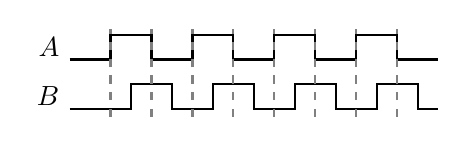
\begin{tikzpicture}[x=0.52cm,y=0.52cm,thick]

% Labels
\node[left] at (0,1.7) {$A$};
\node[left] at (0,0.5) {$B$};

% A
\draw
(0,1.4) --
(1,1.4) --
(1,2.0) --
(2,2.0) --
(2,1.4) --
(3,1.4) --
(3,2.0) --
(4,2.0) --
(4,1.4) --
(5,1.4) --
(5,2.0) --
(6,2.0) --
(6,1.4) --
(7,1.4) --
(7,2.0) --
(8,2.0) --
(8,1.4) --
(9,1.4);

% B
\draw
(0,0.2) --
(1.5,0.2) --
(1.5,0.8) --
(2.5,0.8) --
(2.5,0.2) --
(3.5,0.2) --
(3.5,0.8) --
(4.5,0.8) --
(4.5,0.2) --
(5.5,0.2) --
(5.5,0.8) --
(6.5,0.8) --
(6.5,0.2) --
(7.5,0.2) --
(7.5,0.8) --
(8.5,0.8) --
(8.5,0.2) --
(9,0.2);

% Timing guides
\foreach \x in {1,2,3,4,5,6,7,8}{
    \draw[dashed,gray] (\x,0) -- (\x,2.15);
}

\end{tikzpicture}

\vspace{0.05cm}

\textbf{FIGURE 3--79}
\end{center}


%===========================================================
% Section 3-2, Exercise 7
%===========================================================

\item \textbf{[Section 3-2, Exercise 7]}
The input waveforms applied to a 3-input AND gate are as indicated
in Figure 3--80. Show the output waveform in proper relation to the
inputs with a timing diagram.

\vspace{0.15cm}

\begin{center}
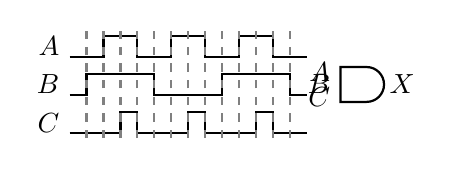
\begin{tikzpicture}[x=0.43cm,y=0.44cm,thick]

\node[left] at (0,2.6) {$A$};
\node[left] at (0,1.5) {$B$};
\node[left] at (0,0.4) {$C$};

% A waveform
\draw
(0,2.3) --
(1,2.3) --
(1,2.9) --
(2,2.9) --
(2,2.3) --
(3,2.3) --
(3,2.9) --
(4,2.9) --
(4,2.3) --
(5,2.3) --
(5,2.9) --
(6,2.9) --
(6,2.3) --
(7,2.3);

% B waveform
\draw
(0,1.2) --
(0.5,1.2) --
(0.5,1.8) --
(2.5,1.8) --
(2.5,1.2) --
(4.5,1.2) --
(4.5,1.8) --
(6.5,1.8) --
(6.5,1.2) --
(7,1.2);

% C waveform
\draw
(0,0.1) --
(1.5,0.1) --
(1.5,0.7) --
(2.0,0.7) --
(2.0,0.1) --
(3.5,0.1) --
(3.5,0.7) --
(4.0,0.7) --
(4.0,0.1) --
(5.5,0.1) --
(5.5,0.7) --
(6.0,0.7) --
(6.0,0.1) --
(7,0.1);

% Guides
\foreach \x in {0.5,1,1.5,2,2.5,3,3.5,4,4.5,5,5.5,6,6.5}{
    \draw[dashed,gray] (\x,-0.05) -- (\x,3.05);
}

% AND gate
\node[and gate US, draw, logic gate inputs=nn,
      scale=0.75] (and1) at (8.6,1.5) {};

\node[left] at (8.0,1.85) {$A$};
\node[left] at (8.0,1.50) {$B$};
\node[left] at (8.0,1.15) {$C$};
\node[right] at (9.15,1.5) {$X$};

\end{tikzpicture}

\vspace{0.05cm}

\textbf{FIGURE 3--80}
\end{center}


%===========================================================
% Section 3-3, Exercise 12
%===========================================================

\item \textbf{[Section 3-3, Exercise 12]}
Repeat Problem 8 for a 4-input OR gate.

\vspace{0.10cm}

\begin{center}
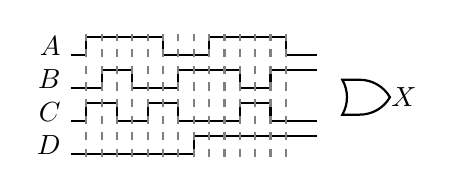
\begin{tikzpicture}[x=0.39cm,y=0.38cm,thick]

\node[left] at (0,3.7) {$A$};
\node[left] at (0,2.6) {$B$};
\node[left] at (0,1.5) {$C$};
\node[left] at (0,0.4) {$D$};

% A
\draw
(0,3.4)--(0.5,3.4)--(0.5,4.0)--(3,4.0)--
(3,3.4)--(4.5,3.4)--(4.5,4.0)--(7,4.0)--
(7,3.4)--(8,3.4);

% B
\draw
(0,2.3)--(1,2.3)--(1,2.9)--(2,2.9)--
(2,2.3)--(3.5,2.3)--(3.5,2.9)--(5.5,2.9)--
(5.5,2.3)--(6.5,2.3)--(6.5,2.9)--(8,2.9);

% C
\draw
(0,1.2)--(0.5,1.2)--(0.5,1.8)--(1.5,1.8)--
(1.5,1.2)--(2.5,1.2)--(2.5,1.8)--(3.5,1.8)--
(3.5,1.2)--(5.5,1.2)--(5.5,1.8)--(6.5,1.8)--
(6.5,1.2)--(8,1.2);

% D
\draw
(0,0.1)--(4,0.1)--(4,0.7)--(8,0.7);

% Guides
\foreach \x in {0.5,1,1.5,2,2.5,3,3.5,4,4.5,5,5.5,6,6.5,7}{
    \draw[dashed,gray] (\x,0) -- (\x,4.1);
}

% OR gate
\node[or gate US, draw, logic gate inputs=nn,
      scale=0.75] at (9.5,2.0) {};

\node[right] at (10.1,2.0) {$X$};

\end{tikzpicture}

\vspace{0.05cm}

\textbf{FIGURE 3--81}
\end{center}


%===========================================================
% Section 3-4, Exercise 17
%===========================================================

\item \textbf{[Section 3-4, Exercise 17]}
For the set of input waveforms in Figure 3--83, determine the output
for the gate shown and draw the timing diagram.

\vspace{0.15cm}

\begin{center}
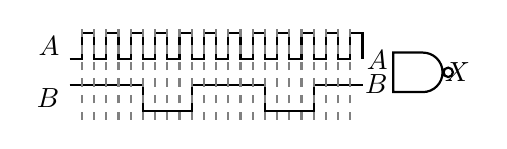
\begin{tikzpicture}[x=0.31cm,y=0.55cm,thick]

\node[left] at (0,1.7) {$A$};
\node[left] at (0,0.5) {$B$};

% Fast clock A
\draw
(0,1.4)
\foreach \x in {0,1,...,11}{
    -- (\x+0.5,1.4)
    -- (\x+0.5,2.0)
    -- (\x+1.0,2.0)
    -- (\x+1.0,1.4)
};

% B
\draw
(0,0.8) --
(3,0.8) --
(3,0.2) --
(5,0.2) --
(5,0.8) --
(8,0.8) --
(8,0.2) --
(10,0.2) --
(10,0.8) --
(12,0.8);

% Timing guides
\foreach \x in {0.5,1,...,11.5}{
    \draw[dashed,gray] (\x,0) -- (\x,2.1);
}

% NAND
\node[nand gate US, draw, logic gate inputs=nn,
      scale=0.85] (nand1) at (14.2,1.1) {};

\node[left] at (13.45,1.38) {$A$};
\node[left] at (13.45,0.82) {$B$};
\node[right] at (14.95,1.1) {$X$};

\end{tikzpicture}

\vspace{0.05cm}

\textbf{FIGURE 3--83}
\end{center}


%===========================================================
% Section 3-4, Exercise 18
%===========================================================

\item \textbf{[Section 3-4, Exercise 18]}
Determine the gate output for the input waveforms in Figure 3--84
and draw the timing diagram.

\vspace{0.15cm}

\begin{center}
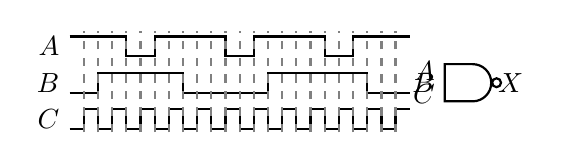
\begin{tikzpicture}[x=0.36cm,y=0.42cm,thick]

\node[left] at (0,2.6) {$A$};
\node[left] at (0,1.5) {$B$};
\node[left] at (0,0.4) {$C$};

% A
\draw
(0,2.9)--(2,2.9)--(2,2.3)--(3,2.3)--
(3,2.9)--(5.5,2.9)--(5.5,2.3)--(6.5,2.3)--
(6.5,2.9)--(9,2.9)--(9,2.3)--(10,2.3)--
(10,2.9)--(12,2.9);

% B
\draw
(0,1.2)--(1,1.2)--(1,1.8)--(4,1.8)--
(4,1.2)--(7,1.2)--(7,1.8)--(10.5,1.8)--
(10.5,1.2)--(12,1.2);

% C
\draw
(0,0.1)--(0.5,0.1)--(0.5,0.7)--(1,0.7)--
(1,0.1)--(1.5,0.1)--(1.5,0.7)--(2,0.7)--
(2,0.1)--(2.5,0.1)--(2.5,0.7)--(3,0.7)--
(3,0.1)--(3.5,0.1)--(3.5,0.7)--(4,0.7)--
(4,0.1)--(4.5,0.1)--(4.5,0.7)--(5,0.7)--
(5,0.1)--(5.5,0.1)--(5.5,0.7)--(6,0.7)--
(6,0.1)--(6.5,0.1)--(6.5,0.7)--(7,0.7)--
(7,0.1)--(7.5,0.1)--(7.5,0.7)--(8,0.7)--
(8,0.1)--(8.5,0.1)--(8.5,0.7)--(9,0.7)--
(9,0.1)--(9.5,0.1)--(9.5,0.7)--(10,0.7)--
(10,0.1)--(10.5,0.1)--(10.5,0.7)--(11,0.7)--
(11,0.1)--(11.5,0.1)--(11.5,0.7)--(12,0.7);

% Guides
\foreach \x in {0.5,1,...,11.5}{
    \draw[dashed,gray] (\x,0) -- (\x,3.05);
}

% NAND
\node[nand gate US, draw, logic gate inputs=nn,
      scale=0.80] at (14,1.5) {};

\node[left] at (13.25,1.85) {$A$};
\node[left] at (13.25,1.50) {$B$};
\node[left] at (13.25,1.15) {$C$};
\node[right] at (14.75,1.5) {$X$};

\end{tikzpicture}

\vspace{0.05cm}

\textbf{FIGURE 3--84}
\end{center}


%===========================================================
% Section 3-5, Exercise 22
%===========================================================

\item \textbf{[Section 3-5, Exercise 22]}
Determine the output waveform in Figure 3--87 and draw the timing
diagram.

\vspace{0.15cm}

\begin{center}
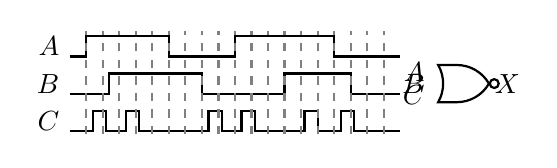
\begin{tikzpicture}[x=0.42cm,y=0.43cm,thick]

\node[left] at (0,2.6) {$A$};
\node[left] at (0,1.5) {$B$};
\node[left] at (0,0.4) {$C$};

% A
\draw
(0,2.3)--(0.5,2.3)--(0.5,2.9)--(3,2.9)--
(3,2.3)--(5,2.3)--(5,2.9)--(8,2.9)--
(8,2.3)--(10,2.3);

% B
\draw
(0,1.2)--(1.2,1.2)--(1.2,1.8)--(4,1.8)--
(4,1.2)--(6.5,1.2)--(6.5,1.8)--(8.5,1.8)--
(8.5,1.2)--(10,1.2);

% C
\draw
(0,0.1)--(0.7,0.1)--(0.7,0.7)--(1.1,0.7)--
(1.1,0.1)--(1.7,0.1)--(1.7,0.7)--(2.1,0.7)--
(2.1,0.1)--(4.2,0.1)--(4.2,0.7)--(4.6,0.7)--
(4.6,0.1)--(5.2,0.1)--(5.2,0.7)--(5.6,0.7)--
(5.6,0.1)--(7.1,0.1)--(7.1,0.7)--(7.5,0.7)--
(7.5,0.1)--(8.2,0.1)--(8.2,0.7)--(8.6,0.7)--
(8.6,0.1)--(10,0.1);

% Guides
\foreach \x in {0.5,1,...,9.5}{
    \draw[dashed,gray] (\x,0) -- (\x,3.05);
}

% NOR gate
\node[nor gate US, draw, logic gate inputs=nn,
      scale=0.80] at (11.8,1.5) {};

\node[left] at (11.05,1.85) {$A$};
\node[left] at (11.05,1.50) {$B$};
\node[left] at (11.05,1.15) {$C$};
\node[right] at (12.55,1.5) {$X$};

\end{tikzpicture}

\vspace{0.05cm}

\textbf{FIGURE 3--87}
\end{center}


%===========================================================
% Section 3-5, Exercise 24
%===========================================================

\item \textbf{[Section 3-5, Exercise 24]}
The NAND and the negative-OR symbols represent equivalent operations,
but they are functionally different. For the NOR symbol, look for at
least one HIGH on the inputs to give a LOW on the output. For the
negative-AND, look for two LOWs on the inputs to give a HIGH output.
Using these two functional points of view, show that both gates in
Figure 3--88 will produce the same output for the given inputs.

\vspace{0.15cm}

\begin{center}
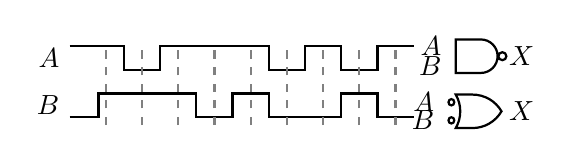
\begin{tikzpicture}[x=0.46cm,y=0.50cm,thick]

\node[left] at (0,1.7) {$A$};
\node[left] at (0,0.5) {$B$};

% A
\draw
(0,2.0)--(1.5,2.0)--(1.5,1.4)--(2.5,1.4)--
(2.5,2.0)--(5.5,2.0)--(5.5,1.4)--(6.5,1.4)--
(6.5,2.0)--(7.5,2.0)--(7.5,1.4)--(8.5,1.4)--
(8.5,2.0)--(9.5,2.0);

% B
\draw
(0,0.2)--(0.8,0.2)--(0.8,0.8)--(3.5,0.8)--
(3.5,0.2)--(4.5,0.2)--(4.5,0.8)--(5.5,0.8)--
(5.5,0.2)--(7.5,0.2)--(7.5,0.8)--(8.5,0.8)--
(8.5,0.2)--(9.5,0.2);

% Guides
\foreach \x in {1,2,3,4,5,6,7,8,9}{
    \draw[dashed,gray] (\x,0) -- (\x,2.1);
}

% NAND
\node[nand gate US, draw, logic gate inputs=nn,
      scale=0.72] at (11.2,1.75) {};

\node[left] at (10.55,2.0) {$A$};
\node[left] at (10.55,1.5) {$B$};
\node[right] at (11.85,1.75) {$X$};

% Negative OR / DeMorgan equivalent
\node[or gate US, draw, logic gate inputs=nn,
      scale=0.72] (negor) at (11.2,0.35) {};

% Input bubbles
\draw (10.54,0.58) circle (0.08);
\draw (10.54,0.12) circle (0.08);

\node[left] at (10.35,0.58) {$A$};
\node[left] at (10.35,0.12) {$B$};
\node[right] at (11.85,0.35) {$X$};

\end{tikzpicture}

\vspace{0.05cm}

\textbf{FIGURE 3--88}
\end{center}


%===========================================================
% Section 3-6, Exercise 26
%===========================================================

\item \textbf{[Section 3-6, Exercise 26]}
Repeat Problem 17 for an exclusive-OR gate.


%===========================================================
% Section 3-6, Exercise 27
%===========================================================

\item \textbf{[Section 3-6, Exercise 27]}
Repeat Problem 17 for an exclusive-NOR gate.

\end{enumerate}

\end{document}